\documentclass[14pt]{extarticle}
\usepackage{fontspec}
\usepackage{polyglossia} % use instead of babel
\usepackage{pgfplots}
\usepackage{float}
\usepackage{amsmath}
\setdefaultlanguage{hebrew}
\setotherlanguage{english}
\newfontfamily\hebrewfont[Script=Hebrew]{Arial}

% TODO: figure out if better to keep this or not, for word document pdf output similarity
\usepackage[margin=1in]{geometry}

% might be useful to ensure similarity to word document pdf output
% \usepackage{setspace}
% \singlespacing

% Reset equation counter at the start of each section
\usepackage{chngcntr}
\usepackage{etoolbox}
\counterwithin*{equation}{section}
\preto{\section}{\setcounter{equation}{0}}

\begin{document}

\begin{center}
    {\LARGE \textbf{ממ"ן 13}}\\
    {\textbf{חוקי ניוטון}}
\end{center}

\begin{itemize}
    \item מגישים: תומר רוזנפלד, שי רואימי
    \item תאריך ביצוע הניסוי: 28 יולי 2025
    \item מדריך הניסוי: ד"ר סילביו ריינהורן
\end{itemize}
\newpage

\section*{ניסוי 1 - החוק הראשון של ניוטיון}
\subsection*{מטרת הניסוי}
בדיקת תוקפו של החוק הראשון של ניוטון
\subsection*{רקע תיאורטי}
החוק הראשון של ניוטון קובע כי גוף ששקול הכוחות עליו הוא אפס נשאר מתמיד במצב מנוחה או בתנועה במהירות קבועה בקו ישר.
\subsection*{מערכת המדידה ומהלך הניסוי}
ראשית איזנו מסילה כך שהייתה אופקית לחלוטין. בדקנו את אופקיות המסילה ע"י הנחת עגלה במקומות שונים על המסילה וראינו שהיא נשארה במקום.  בנוסף בדקנו בעזרת פלס.

בקצה של המסילה חיברנו חיישן תנועה, בניסוי זה  נעזרנו בו למדידת מיקום העגלה.

לאחר מכן דחפנו קלות את העגלה והקלטנו את תוצאות המדידה בתוכנת PASCO Capstone. המדידה הכילה את מיקום העגלה ביחס לזמן התחלת ההקלטה.

\subsection*{תוצאות וניתוח}
הגרף הבא מציג את מיקום העגלה ביחס לזמן: 
\begin{figure}[H]
    \centering
    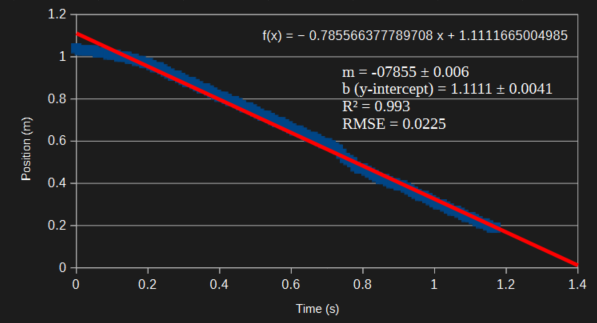
\includegraphics[width=0.8\textwidth]{maman_13_experiment_1_position_time_graph.png}
    \caption{מיקום העגלה ביחס לזמן}
\end{figure}

ניתן לראות שהגרף מתואר היטב ע"י פונקציה ליניארית עם שיפוע $m=0.7856$ ולכן:
\begin{center}
\begin{equation}
\begin{aligned}
    x(t) = x_0 + v_0 t + \frac{1}{2} a t^2 \\
    x_0 = 1.1111 \\
    a = 0 \\
    v_0 = \textbf{שיפוע הגרף} = -0.7856 \\
\end{aligned}
\end{equation}
\end{center}
סימן המינוס הוא מכיוון שכיוון התנועה של העגלה הוא לכיוון חיישן התנועה.

\subsection*{דיון ומסקנות}
בניסוי שקול הכוחות על הגוף בציר התנועה (המסילה) היה אפס וכך יכלננו לבדוק את קיום החוק הראשון של ניוטון.

במדידה קיבלנו גרף מקום ביחס לזמן, עם התאמה טובה לפונקציה ליניארית,  ומשם הסקנו כי מהירות הגוף קבועה - כלומר הגוף מתמיד במצב תנועה במהירות קבועה בקו ישר, כפי שקובע החוק הראשון של ניוטון.

החוסר התאמה הליניארית בגרף יכולה לנבוע מחיכוך, כאשר החיכוך עלול להשתנות גם כתלות במיקום הגוף על המסילה (המסילה אינה חלקה לכל אורכה), וגם אולי משיפוע קל במסילה.

\section*{ניסוי 2 - החוק השני של ניוטון - מסילה משופעת}
\subsection*{מטרת הניסוי}
TODO

\section*{ניסוי 3 - החוק השני של ניוטון - כוח  חופשי}
\subsection*{מטרת הניסוי}
מציאת מסת עגלה בעזרת הפעלת כוח חופשי
\subsection*{רקע תיאורטי}   
כידוע, ע"פ החוק השני שני של ניטון:
\begin{equation}
\Sigma F = m a
\end{equation}
כאשר $\Sigma F$ הוא סכום הכוחות הפועלים על גוף, $m$ היא מסת הגוף ו-$a$ היא תאוצת הגוף.
ניסוי זה מתרחש על מסילה מאוזנת, כך שנתייחס ררק לכוחות בציר האופקי.
וכן בציר האופקי הכוח המרכזי הפועל הוא הכוח שנפעיל בעת דחיפת ומשיכה העגלה ובכן

\begin{equation}
F_{push} = m a
\end{equation}
\subsection*{מערכת המדידה ומהלך הניסוי}
על  מסילה מ אוזנת הרכבנו עגלה וחיישן כוח המחובר לעגלה.
תפסנו בוו של  חיישן הכוח עם היד ודחפנו את העגלה מצד לצד, כאשר במקביל מדדנו  את הכוח והתאוצה  ביחס לזמן (בעזרת החיישן).
\subsection*{תוצאות וניתוח}
הגרף הבא מציג את הכוח ביחס לזמן:
\begin{figure}[H]
    \centering
    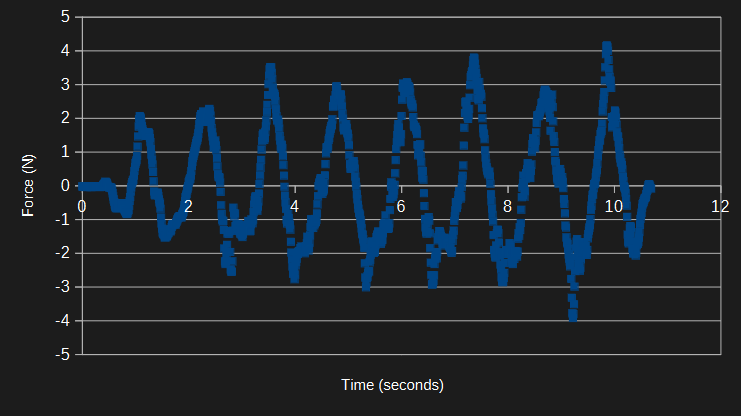
\includegraphics[width=0.8\textwidth]{maman_13_experiment_3_force_to_time.png}
    \caption{כוח ביחס לזמן}
\end{figure}
והגרף הבא מציג את התאוצה ביחס לזמן:
\begin{figure}[H]
    \centering
    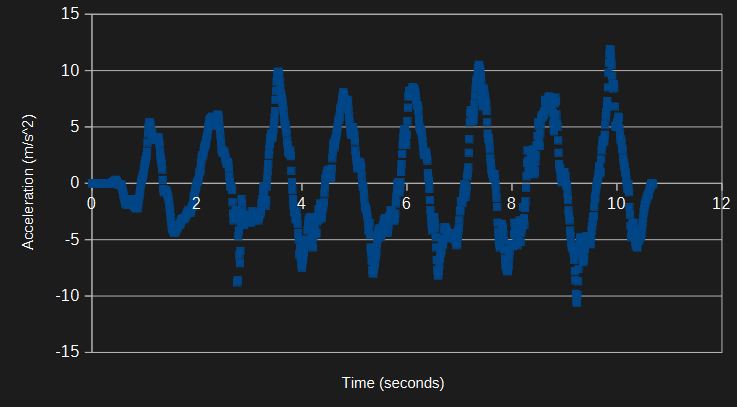
\includegraphics[width=0.8\textwidth]{maman_13_experiment_3_acceleration_to_time.png}
    \caption{תאוצה ביחס לזמן}
\end{figure}

ניתן לראות שכיוון התאוצה וכיוון הכוח משתנים יחד, כפי שציפינו ע"פ החוק השני של ניוטון.
כיוון התאוצה והכוח מתבטא בחיוביות או שליליות הערכים בגרף. כלומר, כאשר העגלה נעה ימינה הכוח והתאוצה חיוביים, וכאשר העגלה נעה שמאלה הכוח והתאוצה שליליים.

הנקודות בהן הכוח והתאוצה שווים לאפס מתארות את הרגע בו העגלה מפסיקה לנועה  לכיוון אחד ומתחילה לנוע לכיוון השני.

ונקודות הקיצון בגרף הכוח מתארות את הרגע בו הכוח המופעל על העגלה הוא מקסימלי באותה דחיפה או משיכה, כלומר הרגע בו הדחיפה או המשיכה של העגלה היא החזקה ביותר, ובהתאם לכך התאוצה היא מקסימלית.

בהמשך ניסוי התבקשנו לייצר גרף של כוח ביחס לתאוצה, כלומר לגרף הבא:
\begin{figure}[H]
    \centering
    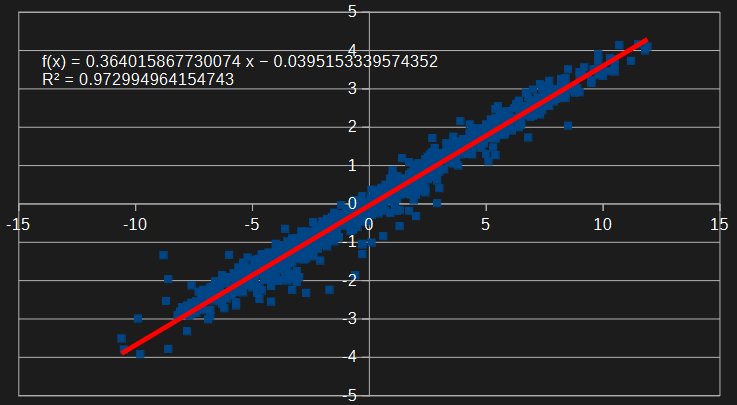
\includegraphics[width=0.8\textwidth]{maman_13_experiment_3_force_to_acceleration.png}
    \caption{כוח ביחס לתאוצה}
\end{figure}

ע"פ נוסחא 2 בסעיף זה, ניתן לייצג את הקשר $m = \frac{F_{push}}{a}$, כלומר שיפוע הגרף הוא מסת העגלה.
את שיפוע מצאנו ע"י התאמה ליניארית וערכו 0.364, כלומר ע"פ המדידה מסת העגלה היא 364 גרם.

שקילת העגלה במשקל החזירה את הערך 355.9 גרם.

\subsection*{דיון ומסקנות}
שקילת העגלה במשקל החזירה את הערך 355.9 גרם, כלומר השגיאה היחסית היא:
\begin{equation}
\text{שגיאה יחסית} = \frac{364 - 355.9}{355.9} \approx 2.7\%
\end{equation}
שגיאה זו עלולה לנבוע כתוצאה מהתעלמות מכוח החיכוך של העגלה במסילה, וכן משגיאה במדידת הכוח או התאוצה.

ההתעלמות מכוח החיכוך מתבטאת במעבר ממשוואה 1 למשוואה 2 בסעיף זה, כאשר קבענו כי $\Sigma F = F_{push}$, כלומר התעלמנו מכוח החיכוך שגם פועל בציר האופקי.

בניסוי זה מדדנו את הכוח המופעל על העגלה ואת התאוצה בעזרת חיישן, וע"י הנתונים שנאספו הצלחנו להראות את היחס הישר בין הכוח מופעיל על העגלה לבין התאוצה שלה, וכן למצוא בקירוב את מסת העגלה, ובכך להראות את קיומו של החוק השני של ניוטון.

\end{document}